\section{Communication Protocol}
\label{cp_sec}

As said in section \ref{adk_sec}, Android Open ADK allows the accessory to exchange generic data with the Android device. A communication protocol is needed to structure this data, in order to allow iNEMO board to correctly communicate with the Android device. At the beginning of this work we had two options for the choice of the protocol:

\begin{itemize}
	\item define a brand new protocol, maybe taking a cue from OpenDMTP\footnote{The OpenDMTP Project: \url{http://www.opendmtp.org}};
	\item adapting the original protocol defined by STM for the communication with the Windows application INEMO Suite.
\end{itemize}

We think that the second option is the best one for the following reasons:

\begin{itemize}
	\item it allows to maintain a continuity whit what has already been developed by STMicroelectronics;
	\item the original protocol is designed to best exploit the features of the board and to fit into the libraries written for it;
	\item it is not useful to write a new protocol that makes the same things that the original one does, but simply with a different format for the exchanged messages.
\end{itemize}

Therefore, an overview of the original protocol is now presented. The messages exchanged by the board have a standard frame that can be described as a sequence of fields in a specific order. The frame format is composed of a header and an optional payload. The header is composed of three mandatory (M) fields, each of which is 1 byte in length, while the payload is an optional field whose maximum length is 61 bytes (this limit can be exceeded by setting the LF/MF field, as explained below). {\bf Figure \ref{fig:frame_format}} shows the general frame format. 

\begin{center}
	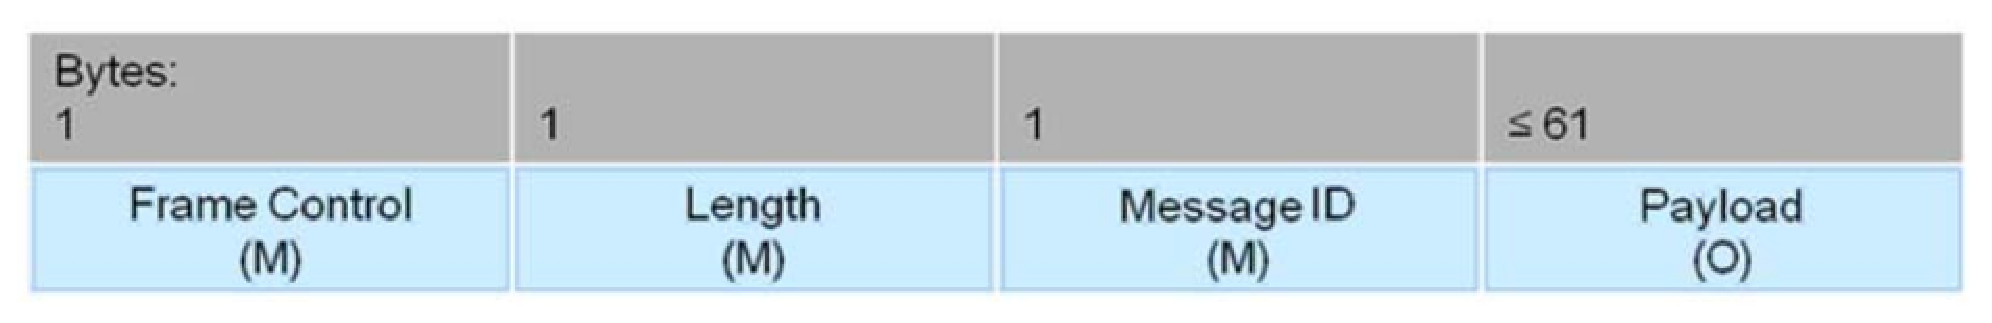
\includegraphics[width=1\linewidth]{pics/frame_format.eps}
	\captionof{figure}{General frame format.}
	\label{fig:frame_format}
\end{center}

The frame control field is 1 byte in length and contains information defining the frame type and other control flags (see {\bf Figure \ref{fig:control_field}}).

\begin{center}
	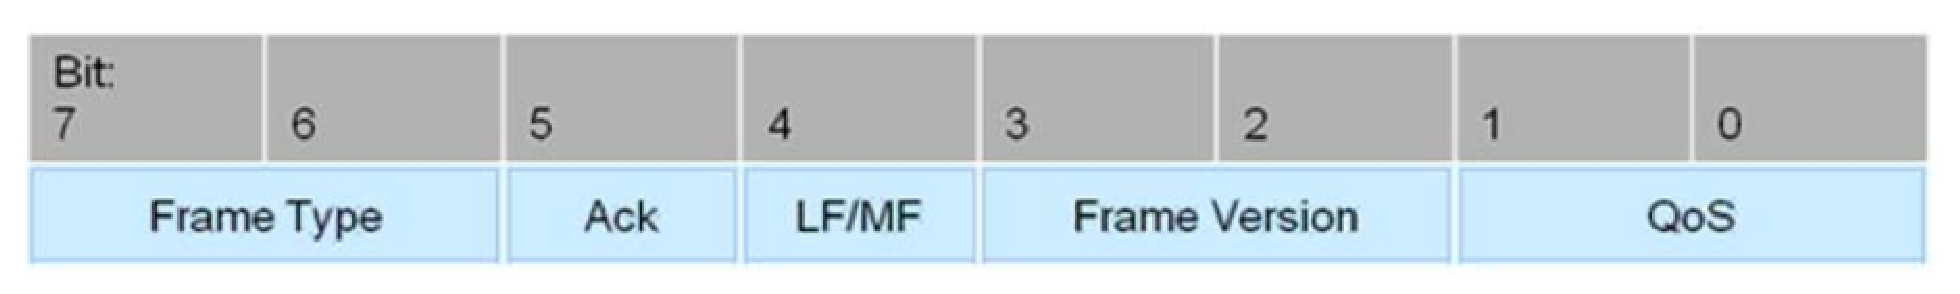
\includegraphics[width=1\linewidth]{pics/control_field.eps}
	\captionof{figure}{Frame control field.}
	\label{fig:control_field}
\end{center}

The frame type subfield is 2 bits in length and is set to one of the values listed in {\bf Table \ref{tab:frame_list}}.

\begin{center}
	\begin{tabularx}{0.9\linewidth}{|>{\centering\arraybackslash}X|>{\centering\arraybackslash}X|}
		\hline
		\textbf{Value} & \textbf{Frame Type} \\
		\hlinewd{1.5pt}
		00 & CONTROL \\
		\hline		
		01 & DATA \\
		\hline
		10 & ACK \\
		\hline
		11 & NACK \\
		\hline
	\end{tabularx}
	\captionof{table}{Frame type list}
	\label{tab:frame_list}
\end{center}

The ACK subfield is 1 bit in length and specifies whether an acknowledgement is required from the recipient on receipt of a DATA or CONTROL frame. If this field is set to one, the recipient sends an acknowledgment frame only if, upon reception, the frame passes all required levels of filtering. If this subfield is set to zero, the recipient device does not send an acknowledgment frame. It is possible to embed a payload in an acknowledgment frame (piggybacking) to send useful information to the transmitter and avoid further transactions. When the ACK field is set to one, and if, upon reception, the frame does not pass the required level of filtering, the recipient sends a no-acknowledgment frame (NACK), whose payload is an error code (e.g. unsupported command, value out of range,...). In the ACK and/or NACK frames the ACK field is set to zero and ignored upon reception.

The LF/MF (last fragment / more fragment) subfield is 1 bit in length and it is used for fragmentation and reassembling. This field is set to zero to indicate a single frame or the last frame of a multiple-frame transaction. This field is set to 1 to indicate that other frames follow, all belonging to the same transaction. 

The frame version subfield is 2 bits in length and is set to ``00'' at this time.

The QoS (Quality of Service) subfield is 2 bits in length and is set to one of the values listed in {\bf Table \ref{tab:qos_list}}. This subfield allows the application to exchange and process data and control frames with different priorities.

\begin{center}
	\begin{tabularx}{0.9\linewidth}{|>{\centering\arraybackslash}X|>{\centering\arraybackslash}X|}
		\hline
		\textbf{Value} & \textbf{QoS} \\
		\hlinewd{1.5pt}
		00 & Normal Priority \\
		\hline		
		01 & Medium Priority \\
		\hline
		10 & High Priority \\
		\hline
	\end{tabularx}
	\captionof{table}{Frame type list}
	\label{tab:qos_list}
\end{center}

Returning to the frame format, the length field is 1 byte in length and contains the number of bytes that follow. Admitted values are in the range 1 to 62.

The message ID is 1 byte in length and contains an identifier used to distinguish the messages.


The frames are classified in four types:

\begin{enumerate}
	\item Communication control frames.
	\item Board information frames.
	\item Sensor setting frames.
	\item Acquisition sensor data frames.
\end{enumerate}

A detailed description of the different frames can be found in the documentation about the Communication Protocol provided by STMicroelectronics\cite{STM_protocol}.



